\documentclass[aspectratio=169,11pt]{beamer}

\usepackage[T1]{fontenc}
\usepackage[utf8]{inputenc}
\usepackage[spanish,es-nodecimaldot]{babel}
\usepackage{newtxtext,newtxmath}
\usepackage{booktabs}
\usepackage{graphicx}
\usepackage{tikz}
\usetikzlibrary{positioning,arrows.meta}
\usepackage{amsmath}

\definecolor{Petroleo}{HTML}{246A73}
\definecolor{Coral}{HTML}{F08A5D}
\definecolor{Tinta}{HTML}{243238}
\definecolor{Nube}{HTML}{F3F6F5}
\definecolor{Gris}{HTML}{657176}

\setbeamercolor{normal text}{fg=Tinta,bg=white}
\setbeamercolor{structure}{fg=Petroleo}
\setbeamercolor{frametitle}{fg=Tinta,bg=white}
\setbeamercolor{title}{fg=white}
\setbeamercolor{subtitle}{fg=white!85}
\setbeamercolor{block title}{fg=white,bg=Petroleo}
\setbeamercolor{block body}{fg=Tinta,bg=Petroleo!6}
\setbeamercolor{alerted text}{fg=Coral!90!black}

\setbeamertemplate{navigation symbols}{}
\setbeamertemplate{itemize item}{\color{Petroleo}$\blacktriangleright$}
\setbeamertemplate{itemize subitem}{\color{Coral}$\bullet$}
\newcommand{\framesource}{}
\setbeamertemplate{frametitle}{%
  \vspace{0.35cm}\insertframetitle\par
  \vspace{0.12cm}{\color{Petroleo}\rule{\textwidth}{1.2pt}}
}
\setbeamertemplate{footline}{%
  \leavevmode%
  \hbox{%
    \begin{beamercolorbox}[wd=.88\paperwidth,ht=2.6ex,dp=1.1ex,left]{author in head/foot}%
      \hspace*{.55cm}\color{Gris}\tiny\framesource
    \end{beamercolorbox}%
    \begin{beamercolorbox}[wd=.12\paperwidth,ht=2.6ex,dp=1.1ex,right,rightskip=.55cm]{date in head/foot}%
      \color{Gris}\scriptsize\insertframenumber/\inserttotalframenumber
    \end{beamercolorbox}%
  }
}
\setbeamertemplate{note page}[plain]
\setbeameroption{hide notes}

\setbeamerfont{title}{size=\fontsize{28}{32},series=\bfseries}
\setbeamerfont{subtitle}{size=\fontsize{15}{18}}
\setbeamerfont{frametitle}{size=\fontsize{22}{25},series=\bfseries}
\setbeamerfont{normal text}{size=\fontsize{12}{15}}

\newcommand{\source}[1]{%
  \gdef\framesource{Fuente: #1}%
}
\newcommand{\metric}[2]{%
  {\color{Petroleo}\fontsize{23}{26}\selectfont\bfseries #1}\par
  \vspace{0.05cm}{\small #2}
}

% Archivo generado automaticamente por scripts/run_analysis.py
\newcommand{\NTotal}{480}
\newcommand{\NTrain}{360}
\newcommand{\NTest}{120}
\newcommand{\ModelAccuracy}{0.733}
\newcommand{\ModelPrecision}{0.794}
\newcommand{\ModelRecall}{0.519}
\newcommand{\ModelFOne}{0.628}
\newcommand{\ModelAUC}{0.724}
\newcommand{\BaselineAccuracy}{0.567}
\newcommand{\TreeDepth}{3}
\newcommand{\TreeLeaves}{8}
\newcommand{\TrueNegative}{61}
\newcommand{\FalsePositive}{7}
\newcommand{\FalseNegative}{25}
\newcommand{\TruePositive}{27}


\title{Árboles de decisión}
\subtitle{Cómo aprende, predice y se evalúa}
\author{Material introductorio reproducible}
\date{Septiembre de 2026}

\begin{document}

% 1 -------------------------------------------------------------------------
\begin{frame}[plain]
  \begin{tikzpicture}[remember picture,overlay]
    \fill[Petroleo] (current page.south west) rectangle (current page.north east);
    \fill[Coral] ([xshift=10.25cm]current page.south west)
      rectangle (current page.north east);
    \draw[white!28,line width=1pt]
      ([xshift=10.8cm,yshift=1.1cm]current page.south west)
      -- ([xshift=12.4cm,yshift=3.0cm]current page.south west)
      -- ([xshift=11.4cm,yshift=5.0cm]current page.south west);
    \fill[white] ([xshift=10.8cm,yshift=1.1cm]current page.south west) circle (3pt);
    \fill[white] ([xshift=12.4cm,yshift=3.0cm]current page.south west) circle (3pt);
    \fill[white] ([xshift=11.4cm,yshift=5.0cm]current page.south west) circle (3pt);
  \end{tikzpicture}
  \vspace{1.2cm}
  \begin{minipage}{0.64\textwidth}
    \usebeamerfont{title}\color{white}\inserttitle\par
    \vspace{0.35cm}
    \usebeamerfont{subtitle}\color{white!88}\insertsubtitle\par
    \vspace{1.25cm}
    {\color{white}\small Caso: \NTotal{} observaciones simuladas y un árbol reproducible.}
  \end{minipage}
  \note{Abrir con la idea central: un árbol traduce una predicción en preguntas que podemos seguir. Aclarar desde el inicio que el caso es completamente simulado y educativo. [Sources] Breiman et al. (1984); repositorio local del ejemplo.}
\end{frame}

% 2 -------------------------------------------------------------------------
\begin{frame}{Un árbol aprende una secuencia de preguntas}
  \vspace{0.3cm}
  \begin{center}
  \resizebox{0.78\textwidth}{!}{%
  \begin{tikzpicture}[
    node distance=1.25cm and 2.0cm,
    every node/.style={font=\small,align=center},
    question/.style={draw=Petroleo,very thick,rounded corners=2pt,fill=Petroleo!7,minimum width=4.1cm,minimum height=1.0cm},
    leaf/.style={draw=Coral,very thick,rounded corners=2pt,fill=Coral!8,minimum width=3.0cm,minimum height=0.9cm},
    edge from parent/.style={draw=Gris,thick,-{Latex[length=2mm]}}
  ]
    \node[question] (root) {¿La edad supera\\un umbral?};
    \node[question,below left=of root] (left) {¿La presión es\\elevada?};
    \node[question,below right=of root] (right) {¿El colesterol\\supera el umbral?};
    \node[leaf,below left=of left] (l1) {Hoja: clase 0};
    \node[leaf,below right=of left] (l2) {Hoja: clase 1};
    \node[leaf,below left=of right] (r1) {Hoja: clase 0};
    \node[leaf,below right=of right] (r2) {Hoja: clase 1};
    \path (root) edge node[left]{sí} (left)
                 edge node[right]{no} (right);
    \path (left) edge (l1) edge (l2);
    \path (right) edge (r1) edge (r2);
  \end{tikzpicture}%
  }
  \end{center}
  \vspace{0.15cm}
  \begin{block}{Idea central}
    Cada división busca grupos más homogéneos; cada hoja entrega una predicción.
  \end{block}
  \source{Breiman et al. (1984).}
  \note{Explicar la lectura de arriba hacia abajo. Las preguntas y umbrales no los programa una persona: el algoritmo los aprende de los datos de entrenamiento. [Sources] Breiman et al. (1984), capítulos 2 y 3.}
\end{frame}

% 3 -------------------------------------------------------------------------
\begin{frame}{La respuesta determina el tipo de árbol}
  \vspace{0.35cm}
  \begin{columns}[T,onlytextwidth]
    \begin{column}{0.47\textwidth}
      {\color{Petroleo}\Large\bfseries Clasificación}\par
      \vspace{0.2cm}
      Predice una \textbf{categoría}.\par
      \vspace{0.35cm}
      \begin{itemize}
        \item riesgo alto o bajo;
        \item diagnóstico A, B o C;
        \item evento sí o no.
      \end{itemize}
      \vspace{0.25cm}
      \colorbox{Petroleo!8}{\parbox{0.91\linewidth}{Criterios habituales: Gini o entropía.}}
    \end{column}
    \begin{column}{0.47\textwidth}
      {\color{Coral!90!black}\Large\bfseries Regresión}\par
      \vspace{0.2cm}
      Predice una \textbf{cantidad continua}.\par
      \vspace{0.35cm}
      \begin{itemize}
        \item concentración;
        \item tiempo de estancia;
        \item costo esperado.
      \end{itemize}
      \vspace{0.25cm}
      \colorbox{Coral!10}{\parbox{0.91\linewidth}{Criterio habitual: reducción del error cuadrático.}}
    \end{column}
  \end{columns}
  \vfill
  Nuestro ejemplo es de \textbf{clasificación binaria}: \texttt{riesgo\_alto} vale 0 o 1.
  \source{Ma (2018), cap. 3; Breiman et al. (1984).}
  \note{Contrastar el tipo de salida, no la forma del árbol. La mecánica de preguntas se conserva; cambia lo que predice la hoja y el criterio usado para dividir. [Sources] Ma (2018), capítulo 3; Breiman et al. (1984).}
\end{frame}

% 4 -------------------------------------------------------------------------
\begin{frame}{Raíz, nodos, ramas y hojas forman reglas legibles}
  \begin{center}
    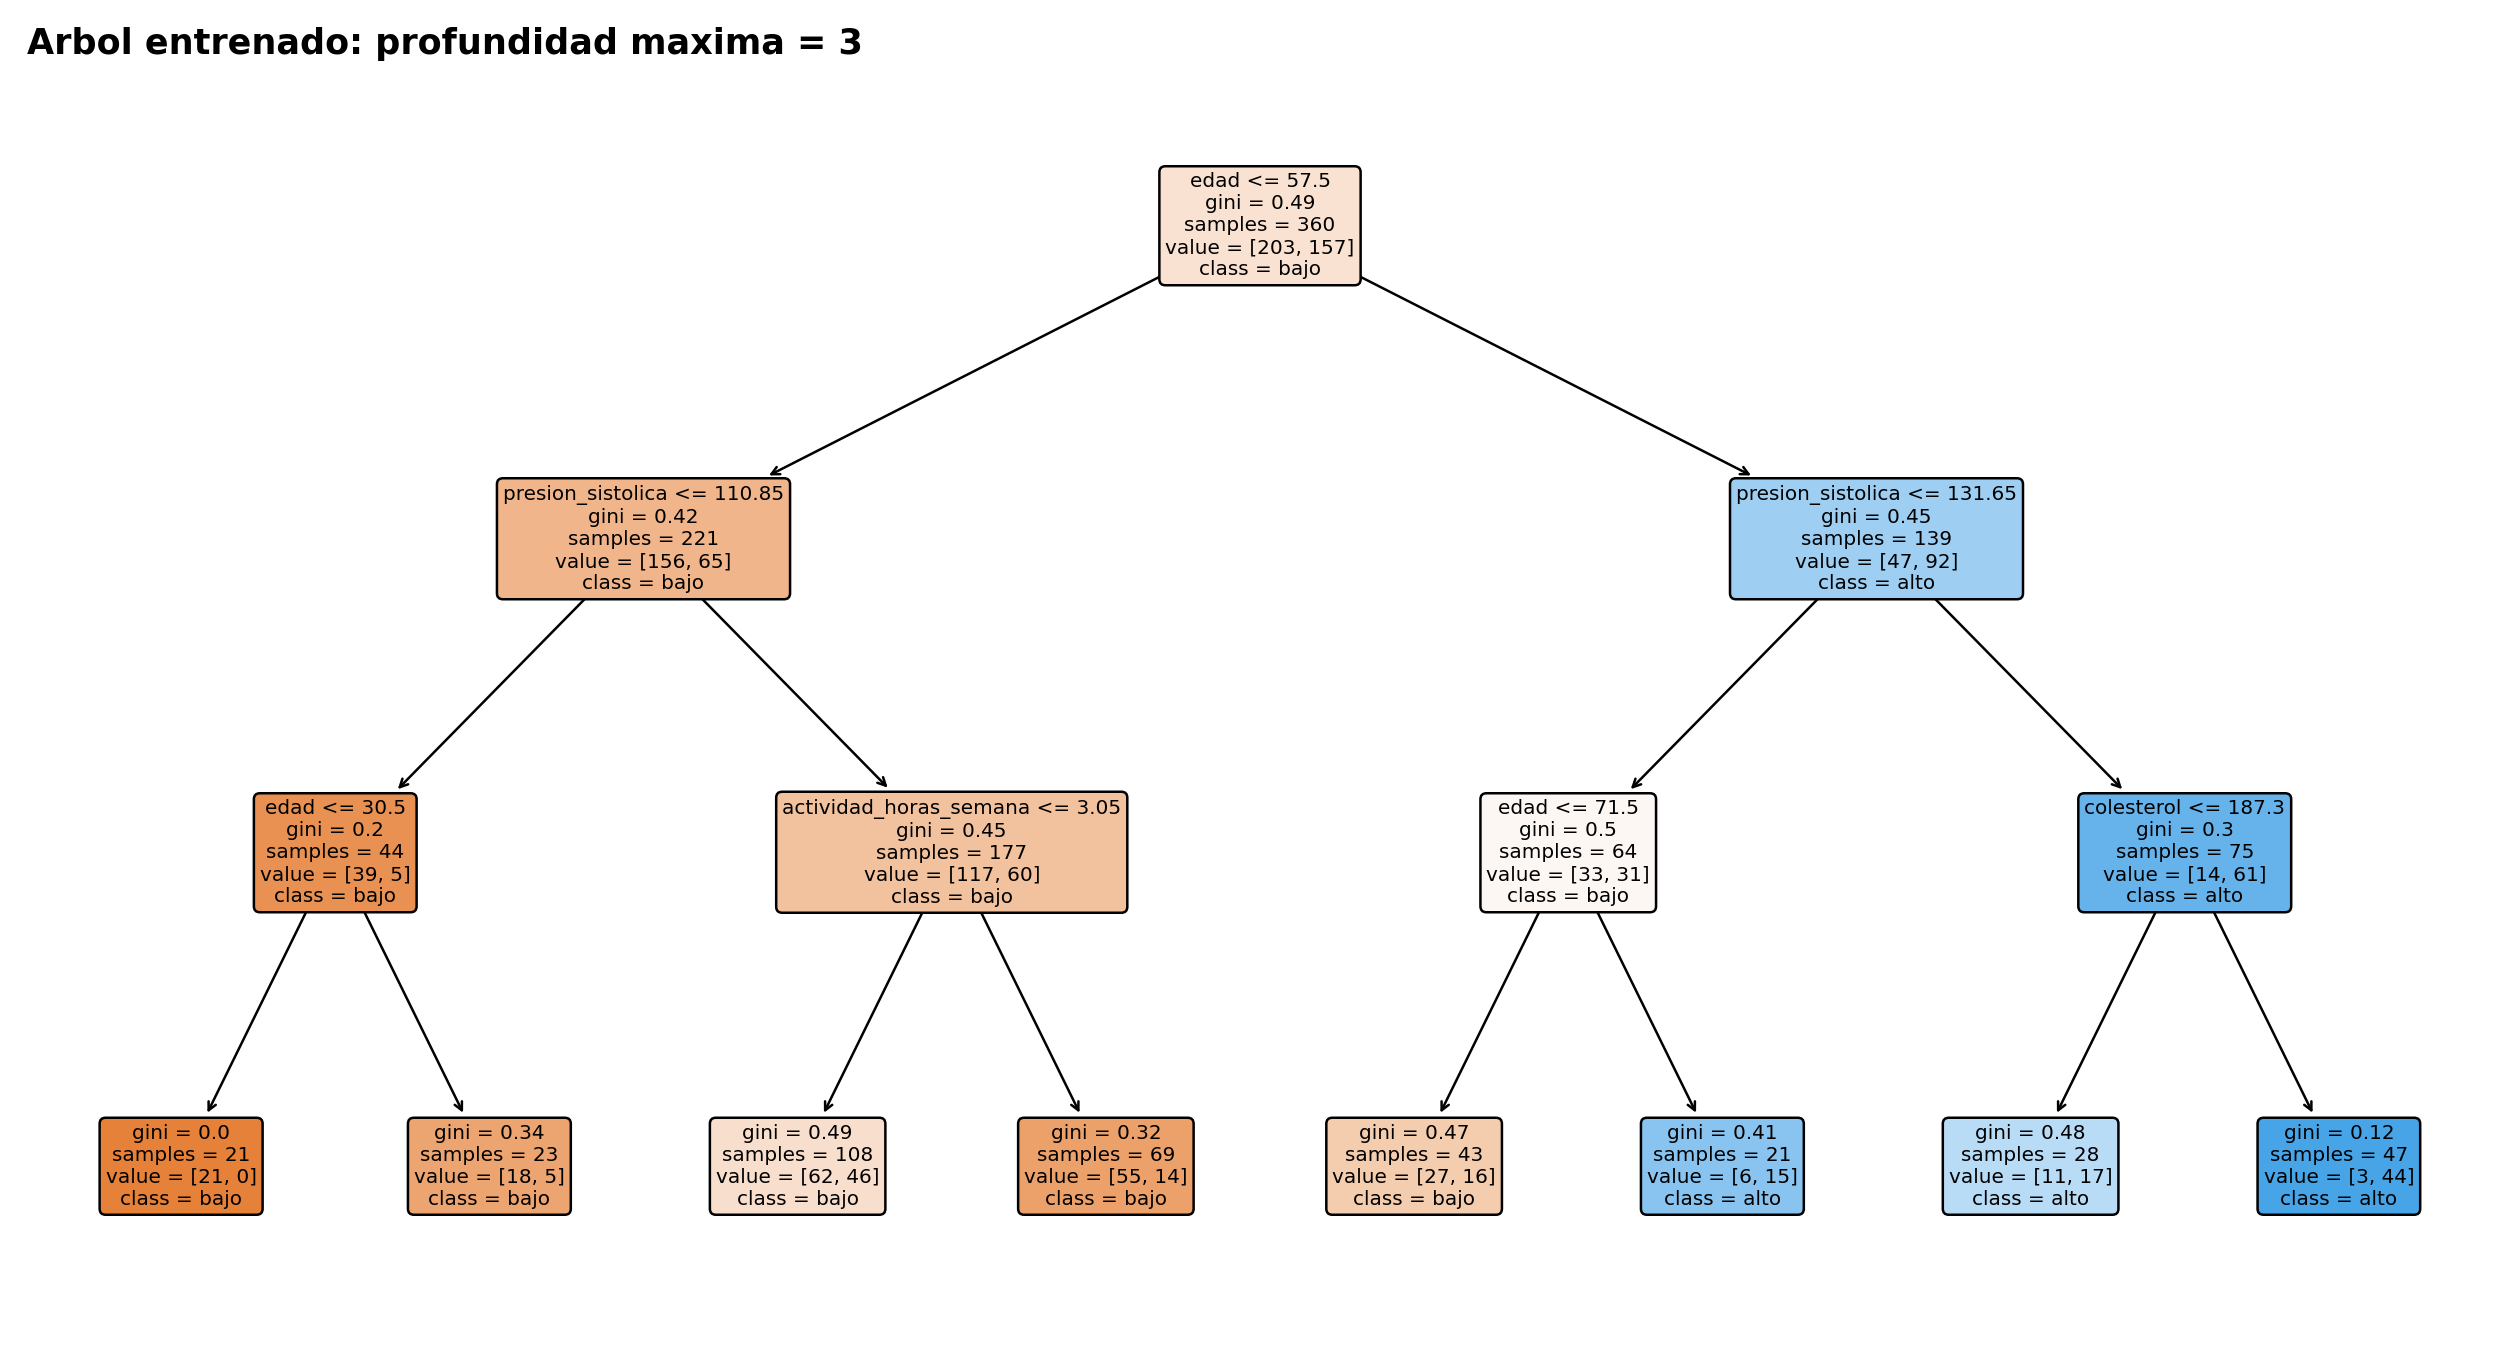
\includegraphics[width=0.84\textwidth,height=0.50\textheight,keepaspectratio]{../figures/decision_tree.png}
  \end{center}
  \vspace{-0.05cm}
  \centering\small Verdadero $\rightarrow$ izquierda · Falso $\rightarrow$ derecha · En la hoja, \texttt{class} es la predicción.
  \source{Pipeline local; datos simulados.}
  \note{Recorrer una sola ruta completa. Señalar samples, value y class. Evitar leer todos los nodos: el objetivo es enseñar el mecanismo, no memorizar el árbol. [Sources] Resultado reproducido en el repositorio local.}
\end{frame}

% 5 -------------------------------------------------------------------------
\begin{frame}{Gini mide cuánta mezcla queda en un nodo}
  \begin{columns}[c,onlytextwidth]
    \begin{column}{0.42\textwidth}
      \begin{block}{Impureza de Gini}
        \[
          G(t)=1-\sum_{k=1}^{K}p_{k,t}^{2}
        \]
      \end{block}
      \vspace{0.25cm}
      El árbol compara preguntas y conserva la que produce la \textbf{mayor reducción de impureza}.
    \end{column}
    \begin{column}{0.53\textwidth}
      \begin{tikzpicture}[x=0.73cm,y=0.73cm]
        \node[anchor=west,font=\bfseries] at (0,5.5) {Nodo puro: $G=0$};
        \foreach \x in {0,...,7} {\fill[Petroleo] (\x,4.7) circle (0.23);}
        \node[anchor=west,font=\bfseries] at (0,3.4) {Mezcla 50/50: $G=0.5$};
        \foreach \x in {0,...,3} {\fill[Petroleo] (\x,2.6) circle (0.23);}
        \foreach \x in {4,...,7} {\fill[Coral] (\x,2.6) circle (0.23);}
        \node[anchor=west,font=\bfseries] at (0,1.3) {Dos hijos puros: $G_{div}=0$};
        \foreach \x in {0,...,3} {\fill[Petroleo] (\x,0.5) circle (0.23);}
        \draw[Gris,thick] (4.0,0.05) -- (4.0,0.95);
        \foreach \x in {5,...,8} {\fill[Coral] (\x,0.5) circle (0.23);}
      \end{tikzpicture}
    \end{column}
  \end{columns}
  \source{Breiman et al. (1984).}
  \note{Calcular oralmente el caso 50/50: 1 menos 0.5 al cuadrado menos 0.5 al cuadrado es 0.5. Un nodo puro tiene Gini cero. [Sources] Breiman et al. (1984).}
\end{frame}

% 6 -------------------------------------------------------------------------
\begin{frame}{Separar antes de aprender protege la evaluación}
  \vspace{0.55cm}
  \begin{columns}[c,onlytextwidth]
    \begin{column}{0.24\textwidth}
      \centering
      {\color{Petroleo}\fontsize{28}{31}\selectfont\bfseries \NTotal}\par
      \vspace{0.12cm}\large casos simulados
    \end{column}
    \begin{column}{0.06\textwidth}
      \centering{\color{Gris}\Large$\longrightarrow$}
    \end{column}
    \begin{column}{0.24\textwidth}
      \centering
      {\color{Petroleo}\fontsize{28}{31}\selectfont\bfseries 75\%}\par
      \vspace{0.12cm}\large entrenamiento\\[-0.1cm]
      \small aprende preguntas
    \end{column}
    \begin{column}{0.06\textwidth}
      \centering{\color{Gris}\Large$\longrightarrow$}
    \end{column}
    \begin{column}{0.24\textwidth}
      \centering
      {\color{Coral!90!black}\fontsize{28}{31}\selectfont\bfseries 25\%}\par
      \vspace{0.12cm}\large prueba\\[-0.1cm]
      \small estima generalización
    \end{column}
  \end{columns}
  \vspace{1.15cm}
  \begin{block}{Regla práctica}
    El conjunto de prueba no debe decidir variables, umbrales ni profundidad.
  \end{block}
  \source{Partición estratificada; semilla 42.}
  \note{Explicar fuga de información: si usamos la prueba para tomar decisiones, deja de representar una evaluación independiente. [Sources] Flujo del repositorio local; práctica estándar de evaluación predictiva.}
\end{frame}

% 7 -------------------------------------------------------------------------
\begin{frame}{El caso usa datos simulados y un árbol pequeño}
  \begin{columns}[c,onlytextwidth]
    \begin{column}{0.52\textwidth}
      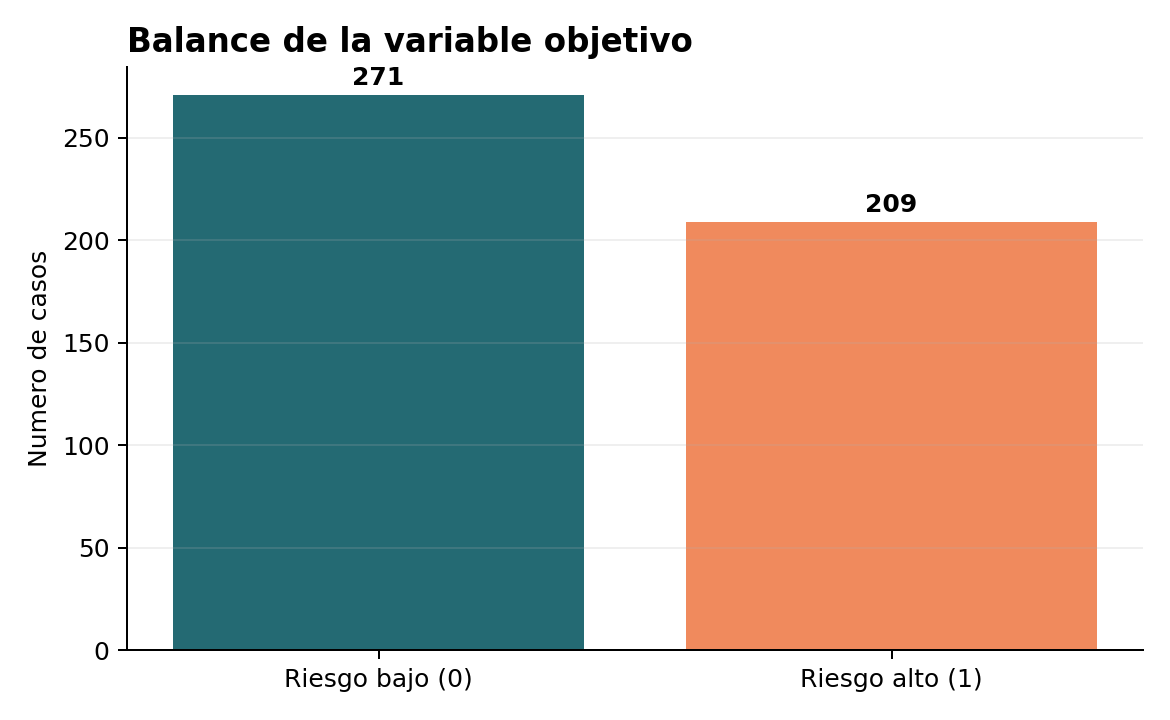
\includegraphics[width=\linewidth]{../figures/class_balance.png}
    \end{column}
    \begin{column}{0.43\textwidth}
      {\color{Petroleo}\Large\bfseries Seis predictores}\par
      \vspace{0.2cm}
      \begin{itemize}
        \item edad y presión sistólica;
        \item colesterol;
        \item fumador;
        \item actividad semanal;
        \item antecedente familiar.
      \end{itemize}
      \vspace{0.22cm}
      \colorbox{Nube}{\parbox{0.91\linewidth}{\small Profundidad máxima: \TreeDepth{}\\Hojas resultantes: \TreeLeaves{}}}
    \end{column}
  \end{columns}
  \source{Datos simulados generados con semilla fija.}
  \note{Aclarar que la relación entre variables y desenlace contiene ruido, por lo que el problema no es perfectamente separable. [Sources] scripts/generate_data.py y output/results/metrics.json.}
\end{frame}

% 8 -------------------------------------------------------------------------
\begin{frame}{La exactitud mejora, pero se pierden positivos}
  \begin{columns}[c,onlytextwidth]
    \begin{column}{0.50\textwidth}
      \centering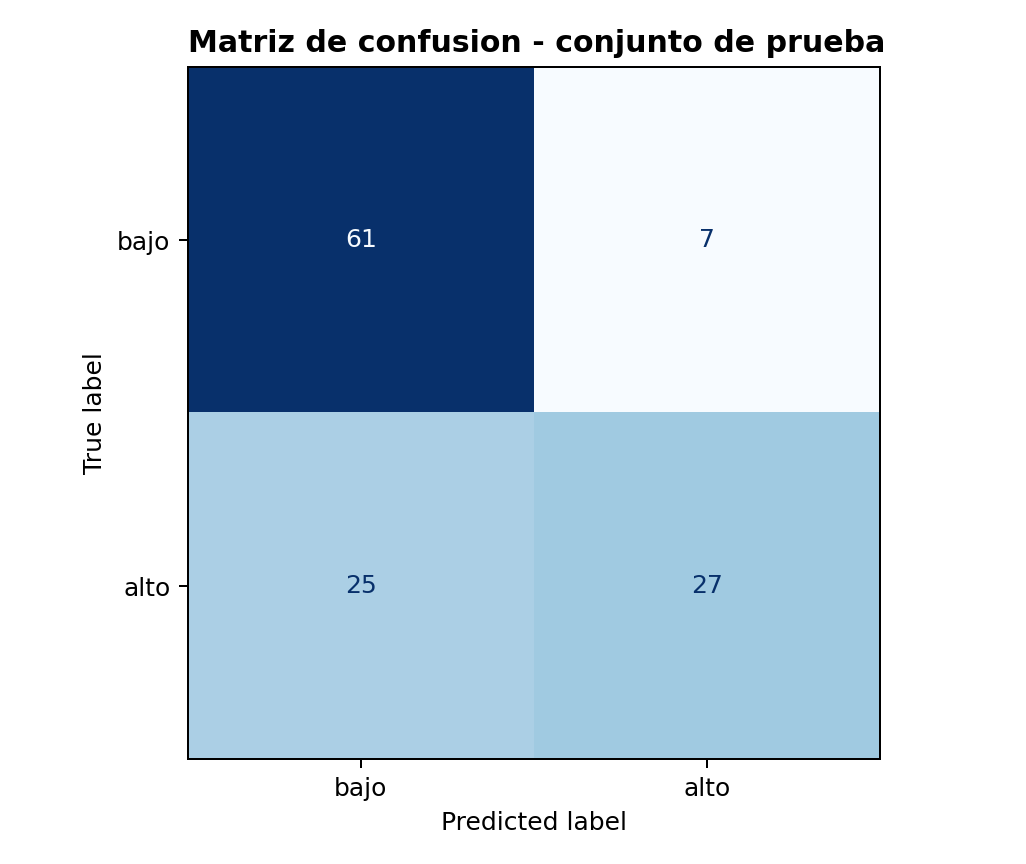
\includegraphics[width=0.88\linewidth]{../figures/confusion_matrix.png}
    \end{column}
    \begin{column}{0.46\textwidth}
      \begin{columns}[T,totalwidth=\linewidth]
        \begin{column}{0.46\linewidth}\metric{\ModelAccuracy}{Exactitud}\end{column}
        \begin{column}{0.46\linewidth}\metric{\ModelPrecision}{Precisión}\end{column}
      \end{columns}
      \vspace{0.55cm}
      \begin{columns}[T,totalwidth=\linewidth]
        \begin{column}{0.46\linewidth}\metric{\ModelRecall}{Sensibilidad}\end{column}
        \begin{column}{0.46\linewidth}\metric{\ModelAUC}{ROC AUC}\end{column}
      \end{columns}
      \vspace{0.55cm}
      {\small Referencia por clase mayoritaria: \textbf{\BaselineAccuracy}.}\par
      \vspace{0.25cm}
      \colorbox{Coral!10}{\parbox{0.93\linewidth}{\small Hay \FalseNegative{} falsos negativos: la exactitud por sí sola no basta.}}
    \end{column}
  \end{columns}
  \source{Conjunto de prueba: $n=\NTest$.}
  \note{Leer primero la matriz: 61 verdaderos negativos, 27 verdaderos positivos, 7 falsos positivos y 25 falsos negativos. Después conectar con sensibilidad. [Sources] output/results/metrics.json y confusion_matrix.csv.}
\end{frame}

% 9 -------------------------------------------------------------------------
\begin{frame}{Más profundidad mejora el ajuste, no siempre la generalización}
  \begin{columns}[c,onlytextwidth]
    \begin{column}{0.67\textwidth}
      \centering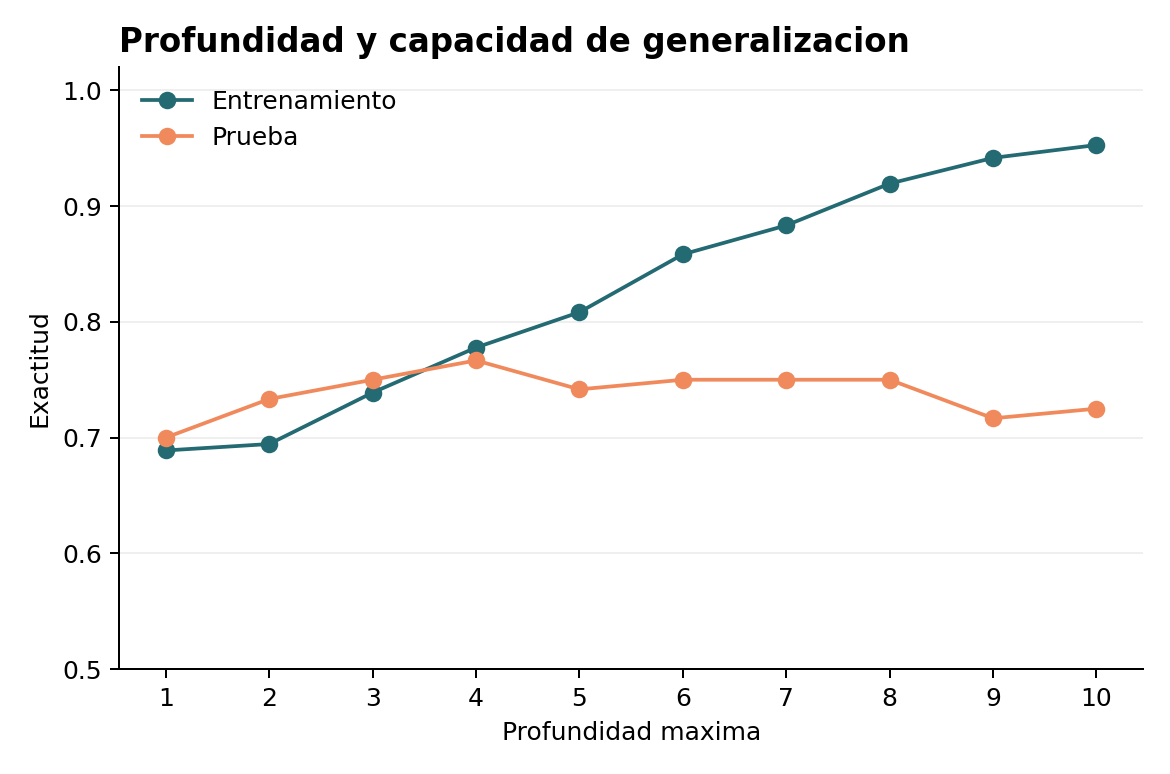
\includegraphics[width=0.84\linewidth]{../figures/depth_curve.png}
    \end{column}
    \begin{column}{0.29\textwidth}
      {\color{Petroleo}\Large\bfseries Controlar complejidad}\par
      \vspace{0.35cm}
      \begin{itemize}
        \item limitar profundidad;
        \item exigir hojas más grandes;
        \item podar ramas;
        \item validar parámetros.
      \end{itemize}
      \vspace{0.2cm}
      \colorbox{Petroleo!8}{\parbox{0.92\linewidth}{\small Señal: entrenamiento mejora; prueba se estanca.}}
    \end{column}
  \end{columns}
  \source{Pipeline local; Breiman et al. (1984).}
  \note{No escoger visualmente la mejor profundidad con esta misma prueba final. En un estudio real se usaría validación cruzada o un conjunto de validación. [Sources] Pipeline local; Breiman et al. (1984), poda por costo-complejidad.}
\end{frame}

% 10 ------------------------------------------------------------------------
\begin{frame}{Interpretabilidad no significa confiabilidad automática}
  \begin{columns}[T,onlytextwidth]
    \begin{column}{0.47\textwidth}
      {\color{Petroleo}\Large\bfseries Lo que ofrece}\par
      \vspace{0.25cm}
      \begin{itemize}
        \item reglas visuales y comunicables;
        \item relaciones no lineales;
        \item interacciones entre variables;
        \item clasificación y regresión.
      \end{itemize}
    \end{column}
    \begin{column}{0.47\textwidth}
      {\color{Coral!90!black}\Large\bfseries Lo que exige}\par
      \vspace{0.25cm}
      \begin{itemize}
        \item control del sobreajuste;
        \item evaluación externa;
        \item revisión de sesgos;
        \item distinguir predicción de causalidad.
      \end{itemize}
    \end{column}
  \end{columns}
  \vspace{0.30cm}
  \begin{block}{En contextos clínicos}
    Transparencia, validación, calibración y juicio profesional siguen siendo indispensables.
  \end{block}
  \source{Ma (2018); Breiman et al. (1984).}
  \note{Subrayar que una ruta explica la decisión del modelo, no la causa del desenlace. Los datos simulados solo demuestran el flujo técnico. [Sources] Ma (2018); Breiman et al. (1984).}
\end{frame}

% 11 ------------------------------------------------------------------------
\begin{frame}{Tres ideas para llevarse}
  \vspace{0.3cm}
  \begin{enumerate}
    \item[\color{Petroleo}\Large\bfseries 1.] \large Un árbol aprende preguntas que dividen los datos en grupos más homogéneos.
    \vspace{0.45cm}
    \item[\color{Petroleo}\Large\bfseries 2.] \large La evaluación debe usar observaciones que no participaron en el aprendizaje.
    \vspace{0.45cm}
    \item[\color{Petroleo}\Large\bfseries 3.] \large Una regla legible sigue necesitando validación y uso responsable.
  \end{enumerate}
  \vspace{0.65cm}
  {\color{Coral!90!black}\Large\bfseries Del árbol al notebook}\par
  \small El repositorio permite reproducir datos, código, figuras y resultados paso a paso.
  \vfill
  {\color{Gris}\tiny
    Lecturas: Breiman, Friedman, Olshen y Stone (1984), \emph{Classification and Regression Trees}.\quad
    Ma (2018), \emph{Using Classification and Regression Trees}, cap. 3.}
  \source{Breiman et al. (1984); Ma (2018), cap. 3.}
  \note{Cerrar resolviendo la pregunta inicial. Invitar a abrir el notebook y cambiar max_depth o criterion como práctica. [Sources] Breiman et al. (1984); Ma (2018), capítulo 3; notebook del repositorio.}
\end{frame}

\end{document}
